\documentclass{article}
\usepackage{graphicx}
\usepackage[margin=1.5cm]{geometry}
\usepackage{amsmath}

\begin{document}
\twocolumn

\title{Friday warm-up: Forces I}
\author{Prof. Jordan C. Hanson}

\maketitle

\section{Memory Bank}

\begin{enumerate}
\item $\vec{F}_{\rm net} = m \vec{a}$ ... Newton's Second Law, relating net force, mass, and acceleration.
\item Units of force: 1 N = 1 kg m s$^{-2}$ ... The definition of a Newton of force, like 1 pound.
\item $g = 9.81$ m s$^{-2}$ ... The gravitational acceleration near the Earth's surface.
\end{enumerate}

\section{Chapter 5 - Forces}

\begin{enumerate}
\item Prove that the two $\theta$ in Fig. \ref{fig:1} are equal, using geometric techniques and the properties of triangles. \\ \vspace{4cm}
\item (a) Using Fig. \ref{fig:1}, show that the magnitude of the weight force is $mg$, given the components $w_x$ and $w_y$. (b) Show that, in the limit $\theta \to 90$ degrees, $w_x$ approaches the full weight of the system.  (c) Show that, in the limit $\theta \to 0$ degrees, $w_y$ approaches the full weight of the system. \\ \vspace{5cm}
\item Suppose an object with mass 40 kg is sliding down an incline (Fig. \ref{fig:1}).  In Figure \ref{fig:1}, the weight force $\vec{w}$ is broken into components $\vec{w}_x$ and $\vec{w}_y$.  (a) If $\theta = 30$ degrees, calculate the magnitudes $w_x$ and $w_y$.  (b) What is the net force on the system, assuming there is no friction? (c) If the system slides 0.45 meters starting from rest, what is the final speed? \\ \vspace{4cm}
\item Suppose a 60 kg skiier is sliding down a slope with $\theta = 15$ degrees.  Assume a frictional force of 40 N opposes the motion. (a) What is the net force on the skiier?  (b) What is the acceleration of the skiier? (c)  Starting with an initial velocity of 5 m s$^{-1}$, how far does the skiier travel in 30 seconds? \\ \vspace{4cm}
\end{enumerate}

\begin{figure}
\centering
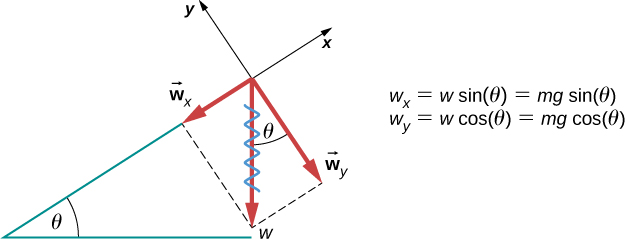
\includegraphics[width=0.5\textwidth]{figures/incline.jpeg}
\caption{\label{fig:1} Forces on an object on an incline.}
\end{figure}


\end{document}
